\documentclass[tikz, border=10pt]{standalone}
\begin{document}
	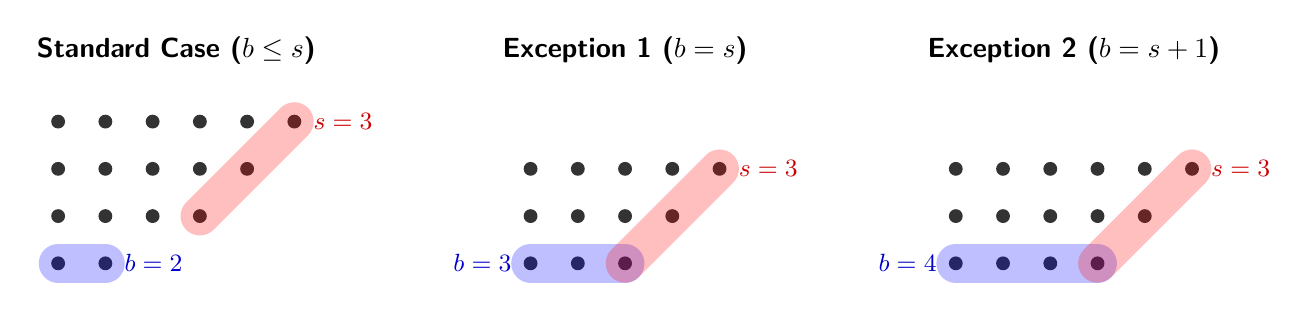
\begin{tikzpicture}[
		scale=0.6,
		dot/.style={circle, fill=black!80, minimum size=5pt, inner sep=0pt},
		highlight base/.style={blue, line width=14pt, opacity=0.25, line cap=round},
		highlight slope/.style={red, line width=14pt, opacity=0.25, line cap=round}
		]
		
		% ---------------------------------------------------------
		% Diagram 1: Standard Case (Base <= Slope)
		% Partition: 6, 5, 4, 2
		% ---------------------------------------------------------
		\begin{scope}[xshift=0cm]
			\node[font=\sffamily\bfseries] at (3.5, 5.5) {Standard Case ($b \le s$)};
			
			% Draw dots
			\foreach \y/\n in {4/6, 3/5, 2/4, 1/2} {
				\foreach \x in {1,...,\n} {
					\node[dot] at (\x, \y) {};
				}
			}
			
			% Highlight Base (y=1)
			\draw[highlight base] (1,1) -- (2,1);
			\node[blue!80!black, right, font=\sffamily\small] at (2.2, 1) {$b=2$};
			
			% Highlight Slope (starts at 6,4 and goes down-left)
			\draw[highlight slope] (6,4) -- (4,2);
			\node[red!80!black, right, font=\sffamily\small] at (6.2, 4) {$s=3$};
		\end{scope}
		
		% ---------------------------------------------------------
		% Diagram 2: Exception 1 (b = s, intersecting)
		% Partition: 5, 4, 3
		% ---------------------------------------------------------
		\begin{scope}[xshift=10cm]
			\node[font=\sffamily\bfseries] at (3, 5.5) {Exception 1 ($b = s$)};
			
			% Draw dots
			\foreach \y/\n in {3/5, 2/4, 1/3} {
				\foreach \x in {1,...,\n} {
					\node[dot] at (\x, \y) {};
				}
			}
			
			% Highlight Base (y=1)
			\draw[highlight base] (1,1) -- (3,1);
			\node[blue!80!black, left, font=\sffamily\small] at (0.8, 1) {$b=3$};
			
			% Highlight Slope (starts at 5,3 and goes down-left)
			\draw[highlight slope] (5,3) -- (3,1);
			\node[red!80!black, right, font=\sffamily\small] at (5.2, 3) {$s=3$};
		\end{scope}
		
		% ---------------------------------------------------------
		% Diagram 3: Exception 2 (b = s + 1, intersecting)
		% Partition: 6, 5, 4
		% ---------------------------------------------------------
		\begin{scope}[xshift=19cm]
			\node[font=\sffamily\bfseries] at (3.5, 5.5) {Exception 2 ($b = s + 1$)};
			
			% Draw dots
			\foreach \y/\n in {3/6, 2/5, 1/4} {
				\foreach \x in {1,...,\n} {
					\node[dot] at (\x, \y) {};
				}
			}
			
			% Highlight Base (y=1)
			\draw[highlight base] (1,1) -- (4,1);
			\node[blue!80!black, left, font=\sffamily\small] at (0.8, 1) {$b=4$};
			
			% Highlight Slope (starts at 6,3 and goes down-left)
			\draw[highlight slope] (6,3) -- (4,1);
			\node[red!80!black, right, font=\sffamily\small] at (6.2, 3) {$s=3$};
		\end{scope}
		
	\end{tikzpicture}
\end{document}